\documentclass[12pt,a4paper]{article}

\usepackage[margin=2.2cm]{geometry}
\usepackage{fontspec}
\setmainfont{Times New Roman}
\usepackage{amsmath,amssymb,bm}
\usepackage{booktabs}
\usepackage{float}
\usepackage{graphicx}
\usepackage{caption}
\usepackage{setspace}
\captionsetup{font=small,labelfont=bf,skip=4pt}
\graphicspath{{figures/}}
\usepackage{hyperref}
\setstretch{1.08}
\raggedbottom

\hypersetup{colorlinks=true,linkcolor=black,urlcolor=blue,pdftitle={}}

\begin{document}

Fig.~4.36(b) adds a reference gain \(H_r\) and a feedforward path \(H_f s\) around the original unity-feedback loop.
Zero steady-state error to a ramp requires both equalities
\begin{equation}
  H_r=1,\qquad H_f=\frac{1}{A}=0.1.
  \label{eq:ideal}
\end{equation}
For the unit parabola \(r(t)=t^2/2\), the steady-state error is then \(\tau/A\), so the acceleration constant is
\begin{equation}
  K_a=\frac{A}{\tau}=10.
  \label{eq:Ka}
\end{equation}

Part~(c) is negative. Any departure of \(H_f\) from \(1/A\) leaves a nonzero constant ramp error, and the system falls back to Type~1.
\(H_r\) is stricter: any departure from 1 leaves no finite steady-state error, and the error grows at a constant slope.
The simulation below, with \(A=10\), \(\tau=1\), and \(r_o=1\), sizes both effects and turns them into tolerance bands that can be written into a specification.
The script is \texttt{type2\_feedforward\_robustness.m}; the printed table is \texttt{steady\_state\_results.txt}.

%==============================================================================
\section{Error transfer function and the ideal Type 2}

The plant is
\[
  G(s)=\frac{A}{s(\tau s+1)}.
\]
Both \(H_r\) and \(H_f s\) enter on the reference path, and the feedback is unity negative feedback, so the loop gain is still \(G(s)\).
The characteristic polynomial
\begin{equation}
  s(\tau s+1)+A=\tau s^2+s+A
  \label{eq:char}
\end{equation}
does not contain \(H_r\) or \(H_f\). Those two parameters change only the numerator of the error, not the poles.

The tracking error \(E=R-Y\) has the transfer function
\begin{equation}
  \frac{E(s)}{R(s)}
  =\frac{\tau s^2+(1-A H_f)s+A(1-H_r)}{s(\tau s+1)+A}.
  \label{eq:EoverR}
\end{equation}
The ramp reference is \(r(t)=r_o t\), so \(R(s)=r_o/s^2\).
The numerator at \(s=0\) is \(A(1-H_r)\), and the coefficient of \(s\) is \(1-A H_f\).

The type for reference inputs is the number of zeros of this numerator at the origin, not the closed-loop poles:
\begin{itemize}
  \item If \(H_r\neq 1\), the numerator has no zero at the origin. The step error is \(1-H_r\), and the ramp error grows linearly in time. For references this is Type~0.
  \item If \(H_r=1\) but \(H_f\neq 1/A\), the numerator has one zero at \(s=0\). The step error is 0 and the ramp error settles to a constant. This is Type~1.
  \item If both equalities hold, the numerator is only \(\tau s^2\), a double zero at the origin. The ramp steady-state error is 0. This is the Type~2 the problem asks for.
\end{itemize}

The last two steady-state values follow from the final-value theorem. With \(H_r=1\) the numerator contributes one factor of \(s\),
\begin{equation}
  e_{ss}
  =\lim_{s\to 0}s\cdot\frac{s\bigl[\tau s+(1-A H_f)\bigr]}{\tau s^2+s+A}\cdot\frac{r_o}{s^2}
  =r_o\Bigl(\frac{1}{A}-H_f\Bigr).
  \label{eq:ess-Hf}
\end{equation}
The ideal point \(H_f=1/A\) makes this zero.

If \(H_r\neq 1\), the dc gain of \(E/R\) is \(1-H_r\), so a ramp remains a ramp. After the transient dies,
\begin{equation}
  e(t)\to (1-H_r)\,r_o\, t+r_o\Bigl(\frac{H_r}{A}-H_f\Bigr).
  \label{eq:asymp}
\end{equation}
The first term is the slope. The second term is the constant that lines the formula up with the simulated curve.
When \(H_r=1\) the slope vanishes and \eqref{eq:asymp} reduces to \eqref{eq:ess-Hf}.

At the ideal parameters, \(E/R=\tau s^2/(\tau s^2+s+A)\).
The unit parabola \(r(t)=t^2/2\) transforms to \(1/s^3\), and its steady-state error is
\[
  e_{ss}
  =\lim_{s\to 0}
   \frac{\tau s^2}{\tau s^2+s+A}\cdot\frac{1}{s^2}
  =\frac{\tau}{A}.
\]
Defining \(e_{ss}=1/K_a\) gives \eqref{eq:Ka}.
This \(K_a\) is defined from the reference error. The loop itself still has only the one integrator in \(G(s)\), and \(\lim_{s\to 0}s^2 G(s)=0\).
The extra order is a cancellation of numerator coefficients, not a second integrator in the loop.

The nominal poles come from \(s^2+s+10=0\): \(\omega_n=\sqrt{10}\approx 3.16~\mathrm{rad/s}\) and \(\zeta=1/(2\sqrt{10})\approx 0.158\).
The oscillation period is about 2~s, and the envelope decays as \(e^{-t/2}\), so the transient is gone after about 8 to 10~s.
Offsets in \(H_r\) and \(H_f\) alone do not move these poles.

%==============================================================================
\section{Simulation results}

The simulation fixes \(A=10\), \(\tau=1\), and \(r_o=1\). The ideal controller is \eqref{eq:ideal}.
The ramp is applied to \eqref{eq:EoverR} with \texttt{lsim} from 0 to 30~s at a step of 0.01~s.
Each offset is a fraction of the ideal value, \(H=H_{\mathrm{ideal}}(1+\delta)\), with \(\delta\) equal to \(0\), \(+1\%\), \(+5\%\), and \(+10\%\).
The two parameters are moved separately: \(H_f\) is held at 0.1 while \(H_r\) moves, then \(H_r\) is held at 1 while \(H_f\) moves.

The value at 30~s has to be read in two ways. When \(H_r=1\) the transient is gone, so \(e(30)\) is \(e_{ss}\).
When \(H_r\neq 1\) the error is still climbing at a constant slope, so \(e(30)\) is only the value at that instant and keeps changing if the run is longer.
The column ``asymptotic \(e(30)\)'' is \eqref{eq:asymp} evaluated at \(t=30\).
Over the eight cases, the simulated endpoint and this asymptote differ by at most \(6.071\times 10^{-8}\).
That residual is the same order as \(e^{-30/2}\): leftover transient, not an error in the formula.
The curves are Fig.~\ref{fig:e}. The endpoints match \texttt{steady\_state\_results.txt}.

\subsection{Offset in \texorpdfstring{\(H_r\)}{Hr}}

\(H_f\) stays at 0.1. The numbers are Table~\ref{tab:Hr}; the curves are the upper plot of Fig.~\ref{fig:e}.

\begin{table}[H]
  \centering
  \caption{\(H_f=0.1\) fixed, \(H_r\) above the ideal value. Slope and asymptote from \eqref{eq:asymp}, with \(r(30)=30\).}
  \label{tab:Hr}
  \begin{tabular}{cccccc}
    \toprule
    Offset & \(H_r\) & Slope & Asymptotic \(e(30)\) & Simulated \(e(30)\) & \(e(30)/r(30)\) \\
    \midrule
    \(0\%\)   & 1.00 & \(0\)      & \(0\)      & \(0\)      & \(0\) \\
    \(+1\%\)  & 1.01 & \(-0.010\) & \(-0.299\) & \(-0.299\) & \(-1.00\%\) \\
    \(+5\%\)  & 1.05 & \(-0.050\) & \(-1.495\) & \(-1.495\) & \(-4.98\%\) \\
    \(+10\%\) & 1.10 & \(-0.100\) & \(-2.990\) & \(-2.990\) & \(-9.97\%\) \\
    \bottomrule
  \end{tabular}
\end{table}

The ideal curve sits on 0 after about 10~s. The other three become straight lines after the same transient, with slope \(-(H_r-1)\).
On the \(+10\%\) curve the error goes from about \(-1\) near 10~s to \(-2.99\) at 30~s, a drop of about 2 in 20~s, which matches the slope \(-0.1\).

\(e(30)\) is slightly less negative than ``slope \(\times 30\)''. The difference is the constant term in \eqref{eq:asymp}.
For \(+1\%\), the slope term is \(-0.300\) and the constant \(r_o(H_r/A-H_f)=0.001\), which add to \(-0.299\).
The larger the offset, the less this constant matters next to the slope term.
For large \(t\), the relative error therefore satisfies
\[
  \frac{e(t)}{r(t)}\to 1-H_r.
\]
If \(H_r\) is high by a few percent, the ramp is led by about that same percentage for the rest of the run.
\(e<0\) means \(y>r\): the reference gain is high, the command into the plant is strong, and the output runs ahead of the reference.

\subsection{Offset in \texorpdfstring{\(H_f\)}{Hf}}

\(H_r\) stays at 1. The numbers are Table~\ref{tab:Hf}; the curves are the lower plot of Fig.~\ref{fig:e}.

\begin{table}[H]
  \centering
  \caption{\(H_r=1\) fixed, \(H_f\) above the ideal value. \(e_{ss}\) from \eqref{eq:ess-Hf}.}
  \label{tab:Hf}
  \begin{tabular}{ccccc}
    \toprule
    Offset & \(H_f\) & \(A H_f\) & Theoretical \(e_{ss}\) & Simulated \(e(30)\) \\
    \midrule
    \(0\%\)   & 0.100 & 1.00 & \(0\)      & \(0\) \\
    \(+1\%\)  & 0.101 & 1.01 & \(-0.001\) & \(-0.001\) \\
    \(+5\%\)  & 0.105 & 1.05 & \(-0.005\) & \(-0.005\) \\
    \(+10\%\) & 0.110 & 1.10 & \(-0.010\) & \(-0.010\) \\
    \bottomrule
  \end{tabular}
\end{table}

The four transients lie almost on top of each other, with a peak near \(+0.25\) and a valley near \(-0.16\), because the poles did not move.
The steady-state separation is only \(0.001\) to \(0.010\), and on a common vertical scale the transient hides it.
The zoom from \(t=20\) to \(30\)~s shows four horizontal lines at the \(e_{ss}\) values of Table~\ref{tab:Hf}.

From \eqref{eq:ess-Hf}, if \(H_f=(1/A)(1+\beta)\),
\begin{equation}
  e_{ss}=-\frac{r_o}{A}\,\beta=-0.1\,\beta.
  \label{eq:beta}
\end{equation}
\(\beta=+0.10\) gives \(e_{ss}=-0.010\), the same as the simulation.
The error is a constant, so the relative error \(e(t)/r(t)\) goes to 0 as \(1/t\).
At 30~s the \(+10\%\) relative error is only \(-0.010/30\approx -0.033\%\).
Next to the percent-for-percent \(H_r\) error of the previous subsection, the \(H_f\) penalty is smaller by a factor of order \(At\).

The sign has the same origin: a high \(H_f\) injects too much velocity command through the derivative feedforward, and the output leads the reference by a fixed distance.
The formula is linear in a negative offset. Lowering \(H_f\) by \(10\%\) (\(H_f=0.09\)) would give \(e_{ss}=+0.010\), a lag. This run only swept the high side.

\begin{figure}[H]
  \centering
  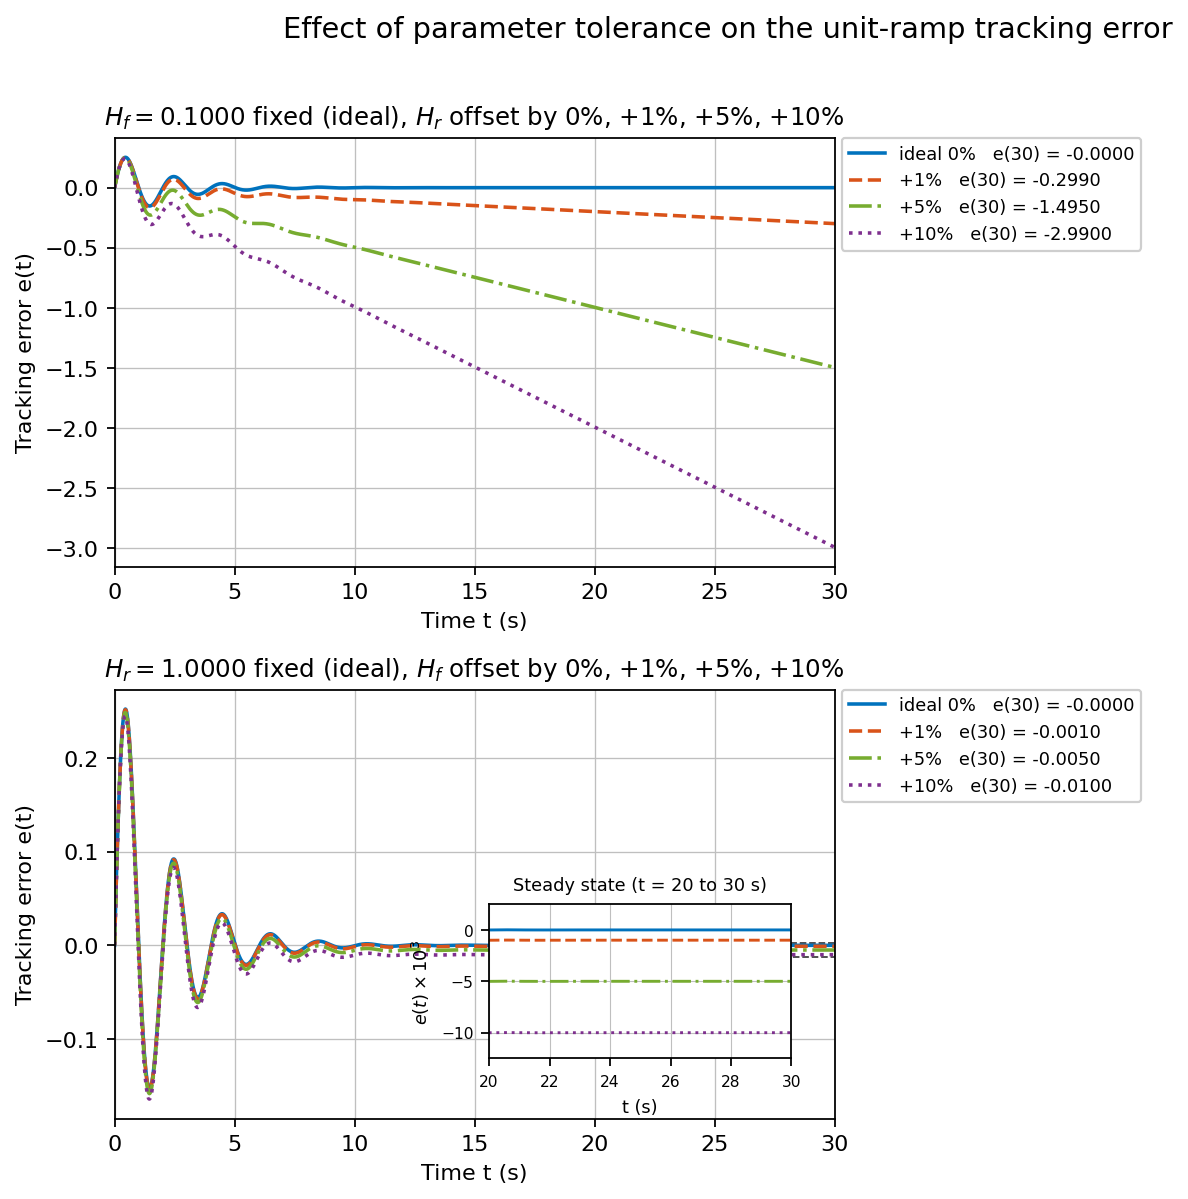
\includegraphics[width=\textwidth]{error_print.png}
  \caption{Tracking error \(e(t)=r(t)-y(t)\) for the unit ramp \(r(t)=t\).
  The upper plot holds \(H_f=0.1\); the lower plot holds \(H_r=1\).
  The inset is \(t=20\) to \(30\)~s, with the vertical axis in units of \(10^{-3}\).
  The legend value \(e(30)\) is the simulated endpoint.}
  \label{fig:e}
\end{figure}

%==============================================================================
\section{Robustness and allowable error}

\subsection{Type 2 has no tolerance band}

Part~(c) asks whether the property survives, not how large the error is.
Type~2 requires the ramp steady-state error to be exactly 0, which is the pair of equalities in \eqref{eq:ideal}.
Any departure of \(H_f\) makes \eqref{eq:ess-Hf} nonzero, and the system returns to Type~1.
The \(+1\%\) row of Table~\ref{tab:Hf} already gives \(e_{ss}=-0.001\neq 0\).
This Type~2 is not robust to \(H_f\), and there is no interval on which a small change still counts as Type~2.

The structural reason is that the extra order comes from the cancellation \(1-A H_f=0\). The loop gain does not contain a second integrator.
If either side of the cancellation drifts, the zero leaves the origin.
The closed-loop roots do not show it. The four \(H_f\) curves oscillate the same way and have the same stability margins, but the ramp error is no longer 0.
Checking only the poles, or only a short transient, misses this tolerance.

The equality for \(H_r\) has no width either. Once it moves, even the Type~1 property that the ramp error stays bounded is lost, and the system is Type~0 for references.
When feedforward is used to create the type, both the reference gain and the feedforward gain are hard equalities.

\subsection{When the specification is an error bound}

A product specification usually does not say ``must be Type~2''. It says the error must not exceed a number.
A tolerance band can then be computed, and the rules for \(H_r\) and \(H_f\) are different.
Set
\[
  H_r=1+\alpha,\qquad H_f=\frac{1}{A}(1+\beta),
\]
where \(\alpha\) and \(\beta\) are relative errors. Substitution into \eqref{eq:asymp} gives
\begin{equation}
  e(t)\to -\alpha\, r_o\, t+\frac{r_o}{A}(\alpha-\beta).
  \label{eq:ab}
\end{equation}

\paragraph{\(H_r\).}
If \(\alpha\neq 0\), the error is unbounded.
No nonzero tolerance on \(H_r\) keeps the ramp error finite for all time.
If the requirement is only \(|e(t)|\le e_{\max}\) over a mission of length \(T\), the slope term dominates,
\begin{equation}
  |\alpha|\le\frac{e_{\max}}{r_o T}.
  \label{eq:tol-Hr-T}
\end{equation}
A longer \(T\) demands a more accurate \(H_r\). For the numbers here, \(r_o=1\), \(e_{\max}=0.30\), and \(T=30~\mathrm{s}\), one gets \(|\alpha|\le 0.01\), which is the \(+1\%\) row of Table~\ref{tab:Hr} (the actual \(|e(30)|\) is 0.299).
The same budget of 0.30 carried out to 300~s forces \(|\alpha|\) down to \(0.001\), that is \(0.1\%\).

If the specification is a relative error \(|e/r|\le\varepsilon\), waiting longer does not help. From \eqref{eq:ab},
\begin{equation}
  |\alpha|\le\varepsilon.
  \label{eq:tol-Hr-rel}
\end{equation}
The relative tolerance on \(H_r\) equals the allowed relative tracking error. A \(1\%\) ramp-tracking spec requires \(H_r\) within \(1\%\), over the whole mission, not at one instant.

\paragraph{\(H_f\).}
With \(\alpha=0\) the error is bounded,
\begin{equation}
  |e_{ss}|=\frac{r_o}{A}\,|\beta|
  \quad\Rightarrow\quad
  |\beta|\le\frac{A}{r_o}\,e_{\max}.
  \label{eq:tol-Hf}
\end{equation}
For \(A=10\) and \(r_o=1\):
\begin{center}
\begin{tabular}{ccc}
  \toprule
  Allowed \(|e_{ss}|\) & \(|H_f-0.1|\) & Relative tolerance \(|\beta|\) \\
  \midrule
  \(0.001\) & \(0.001\) & \(1\%\) \\
  \(0.005\) & \(0.005\) & \(5\%\) \\
  \(0.010\) & \(0.010\) & \(10\%\) \\
  \bottomrule
\end{tabular}
\end{center}
The last row is the \(+10\%\) case of Table~\ref{tab:Hf}.
The relative error shrinks as \(1/t\), so a few percent on \(H_f\) is usually acceptable when only long-term relative accuracy matters. When the absolute lag matters, use \eqref{eq:tol-Hf} instead of copying the \(H_r\) percentage.

\paragraph{Plant-gain drift.}
The simulation holds \(A\) fixed. In practice the condition is the product \(A H_f=1\), so drift in \(A\) and drift in \(H_f\) enter the same expression.
With \(H_r=1\) and \(H_f\) left at its nominal value \(1/A\), an actual gain \(A(1+\gamma)\) gives
\[
  e_{ss}
  =r_o\Bigl(\frac{1}{A(1+\gamma)}-\frac{1}{A}\Bigr)
  =-\frac{r_o}{A}\cdot\frac{\gamma}{1+\gamma}
  \approx-\frac{r_o}{A}\,\gamma.
\]
To first order, a \(10\%\) error in \(A\) and a \(10\%\) error in \(H_f\) are about the same size, and \(|e_{ss}|\) is about \(0.01\).
Setting the feedforward gain accurately is not enough: identification error in the plant gain comes in through the same path. This follows from \eqref{eq:ess-Hf} and was not simulated separately.

\subsection{How to write the specification}

If the specification is literally zero ramp error, neither \(H_r\) nor \(A H_f\) has a tolerance. This Type~2 is not a property that can be manufactured.
Zero error requires the integrators to sit inside the loop, so that the type follows the loop gain instead of a feedforward cancellation.

If the specification is an error bound, the two parameters are written separately:
\begin{enumerate}
  \item For \(H_r\), use \eqref{eq:tol-Hr-rel} or \eqref{eq:tol-Hr-T}. A relative tracking error of a few percent means the same few percent on \(H_r\). A longer mission tightens the absolute-error budget further. Any nonzero deviation has no steady state.
  \item For \(H_f\), and for the plant gain \(A\), use \eqref{eq:tol-Hf}. Divide the allowed constant lag by \(r_o/A\) to get the relative tolerance. Here \(r_o/A=0.1\), so a constant-error budget of \(0.01\) allows \(\pm 10\%\) on \(H_f\).
  \item Acceptance has to look at the ramp error after the transient, not at a step response or at the poles. A steady \(H_f\) error of order \(0.01\) is hidden by a transient peak of about \(0.25\). The record has to cover an interval after the transient has died, with the tail enlarged as in the lower plot of Fig.~\ref{fig:e}.
\end{enumerate}

On these numbers, \(1\%\) on \(H_r\) produces an error of \(-0.299\) at 30~s, while \(1\%\) on \(H_f\) produces only \(-0.001\).
The same \(1\%\) component tolerance is about \(At=300\) times tighter for the reference gain than for the feedforward gain.
The feedforward path can absorb a few percent of manufacturing spread. The reference gain cannot.
\end{document}
